\bookchapter{Reward design}\label{ch:rl5}

\section*{Explanation}
The reward is the only way to tell an RL robot what you want. The robot does \emph{not} understand your intention. It maximises exactly the numbers that you give it, and it is very good at finding unexpected ways to get high numbers. Designing the reward is therefore one of the most important and most difficult parts of robot learning.

\begin{keyidea}[The golden rule]
The robot optimises what you \textbf{reward}, not what you \textbf{mean}. If there is a loophole in the reward, a good learner will find it.
\end{keyidea}

\begin{example}[Loopholes]
Imagine three rewards for a soccer robot:
\begin{itemize}[nosep]
  \item $+1$ in every step in which the ball is less than $1$\,m from the robot. The robot learns to stand next to the ball and never touch it.
  \item $+$ forward speed of the robot's head. The robot learns to throw itself forward: for a moment the head is very fast.
  \item $+1$ every time the foot touches the ball. The robot learns to tap the ball a little again and again instead of dribbling it to the goal.
\end{itemize}
All three robots do exactly what the reward says, but not what the designer meant. This is called \textbf{reward hacking}.
\end{example}

\section*{Sparse and dense rewards}
The most honest reward is the \textbf{sparse} one: $+1$ if a goal is scored, $0$ otherwise. But a robot that has not learned anything moves randomly and practically never scores. It never sees a reward other than $0$, so there is nothing to learn from. A \textbf{dense} (shaped) reward gives feedback in every step, for example ``the closer to the ball the better''.

\begin{center}
\begin{tikzpicture}
\begin{axis}[gr, axis lines=left, xlabel near ticks, ylabel near ticks, width=9.5cm,height=5.6cm, xlabel={distance $d$ to the ball (m)}, ylabel={reward}, xmin=0,xmax=5,ymin=-0.1,ymax=1.2, xtick={0,1,2,3,4,5}, ytick={0,0.5,1}, legend pos=north east]
  \addplot[red,very thick,domain=0:5,samples=200]{(x<0.3)};
  \addlegendentry{sparse: $1$ only at the ball}
  \addplot[blue,very thick,domain=0:5]{1-x/5};
  \addlegendentry{dense: closer is better}
\end{axis}
\end{tikzpicture}
\captionof{figure}{A sparse reward gives a signal only in a tiny region around the ball. A dense reward guides the robot from every distance.}\label{fig:rl5_sparse}
\end{center}

\section*{A reward is a sum of terms}
Real reward functions are sums of weighted terms. Each term pushes the robot towards one wish or away from one problem. For a walking policy typical terms are:

\begin{center}
\renewcommand{\arraystretch}{1.3}
\begin{tabular}{p{4.6cm}p{3.6cm}p{4.6cm}}
\textbf{Term} & \textbf{Sign} & \textbf{Purpose}\\ \hline
velocity tracking & positive & walk at the commanded speed\\
staying upright & positive & the torso should not tilt\\
alive bonus & positive & staying in the game is good\\
torque (energy) & negative & do not waste energy or overheat the motors\\
action rate (jerkiness) & negative & smooth motions that the real motors can follow\\
falling (termination) & large negative & never fall\\
\end{tabular}
\end{center}

\textbf{Tracking terms.} To reward ``close to the commanded speed'' a smooth bump is often used instead of a plain difference:
\[
r_{\text{track}}=\exp\!\left(-\frac{(v_{\text{cmd}}-v)^2}{\sigma^2}\right).
\]
It is $1$ for a perfect match and falls towards $0$ for large errors. The width $\sigma$ decides how forgiving the term is (Figure~\ref{fig:rl5_kernel}).

\begin{center}
\begin{tikzpicture}
\begin{axis}[gr, axis lines=left, xlabel near ticks, ylabel near ticks, width=9.5cm,height=5.6cm, xlabel={speed $v$ (m/s), command $v_{\mathrm{cmd}}=1$}, ylabel={$r_{\mathrm{track}}$}, xmin=0,xmax=2,ymin=0,ymax=1.1, xtick={0,0.5,1,1.5,2}, ytick={0,0.5,1}, legend pos=north east]
  \addplot[blue,thick,domain=0:2,samples=100]{exp(-((1-x)^2)/(0.25^2))};
  \addlegendentry{$\sigma=0.25$}
  \addplot[red,thick,domain=0:2,samples=100]{exp(-((1-x)^2)/(0.5^2))};
  \addlegendentry{$\sigma=0.5$}
\end{axis}
\end{tikzpicture}
\captionof{figure}{The tracking reward for the commanded speed $1$\,m/s. A small $\sigma$ demands precision but gives almost no signal when the robot is far from the target speed.}\label{fig:rl5_kernel}
\end{center}

\begin{example}[Adding up one step]
Let the reward per step be
\[
r=2.0\cdot r_{\text{track}}\;-\;0.001\cdot\sum_{\text{joints}}\tau^2\;+\;0.5 ,
\]
with $\sigma=0.25$ and the command $v_{\text{cmd}}=1$\,m/s. The robot walks at $v=0.8$\,m/s and the sum of the squared joint torques is $400$ (in some units). Then $r_{\text{track}}=\exp(-0.04/0.0625)=0.527$ and
\[
r=2.0\cdot0.527-0.001\cdot400+0.5=1.054-0.4+0.5\approx1.15 .
\]
\end{example}

\section*{Balancing the weights}
The weights decide what the robot prefers. Let us compare four behaviours with the reward above (standing still has a torque sum of only $25$, walking has $400$).

\begin{center}
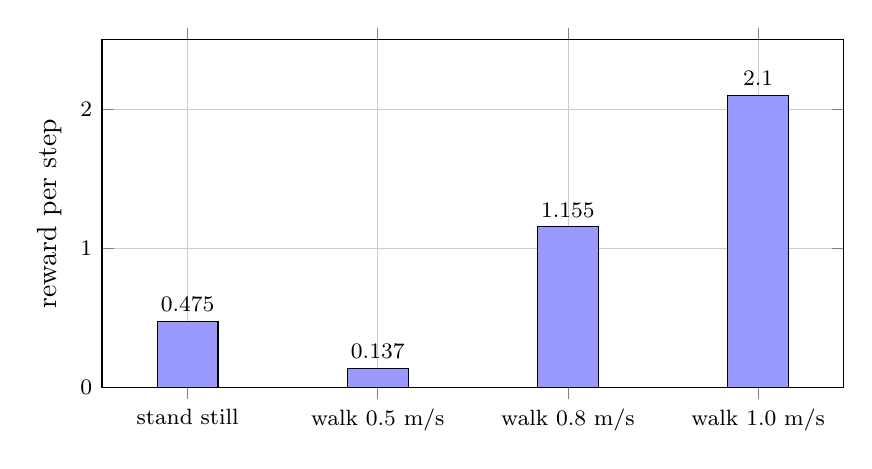
\begin{tikzpicture}
\begin{axis}[ybar, width=11cm,height=6cm, bar width=22pt, ymin=0,ymax=2.5, ylabel={reward per step}, symbolic x coords={stand still,walk 0.5 m/s,walk 0.8 m/s,walk 1.0 m/s}, xtick=data, x tick label style={font=\footnotesize}, tick label style={font=\footnotesize}, nodes near coords, nodes near coords style={font=\footnotesize,/pgf/number format/.cd,fixed,precision=3}, grid=major, grid style={line width=0.2pt,draw=gray!40}, enlarge x limits=0.15]
  \addplot[fill=blue!40] coordinates {(stand still,0.475) (walk 0.5 m/s,0.137) (walk 0.8 m/s,1.155) (walk 1.0 m/s,2.1)};
\end{axis}
\end{tikzpicture}
\captionof{figure}{Reward per step for four behaviours ($\sigma=0.25$). Walking slowly earns \emph{less} than standing still, so a beginner robot will prefer to stand.}\label{fig:rl5_bars}
\end{center}

Standing still earns $0.475$ per step, but walking at only $0.5$\,m/s earns just $0.137$: the tracking reward is almost zero and the torques cost $0.4$. A robot that has just started learning will therefore discover that \emph{standing is better than trying to walk}, and may never learn to walk. There are two typical remedies: use a wider tracking bump ($\sigma=0.5$ gives $2\cdot0.368-0.4+0.5=0.836$ for $0.5$\,m/s, which beats standing) or reduce the torque weight in the beginning.

\begin{keyidea}[Reward design is experimenting]
Start with few terms. Log every term separately during training, watch videos of the robot, and ask: ``which behaviour would earn the highest reward, and is it what I want?'' Change one weight at a time.
\end{keyidea}

\section*{Falling and early termination}
When the robot falls the episode usually ends. This interacts with the sign of the reward.
\begin{itemize}[nosep]
  \item If the rewards per step are \emph{positive}, ending the episode loses all future rewards, so falling is automatically bad.
  \item If the rewards per step are \emph{negative}, ending the episode early \emph{saves} costs, and the robot may learn to fall on purpose!
\end{itemize}

\begin{example}
Each step costs $-0.5$, a fall costs a single penalty of $-10$, and $100$ steps remain ($\gamma=1$). Staying upright until the end gives $100\cdot(-0.5)=-50$. Falling immediately gives only $-10$. The robot prefers to fall. A positive alive bonus fixes this: with $+0.5$ per step staying upright is worth $+50$.
\end{example}

\section*{Potential-based shaping}
Dense rewards can change which behaviour is optimal and create loopholes. There is a safe way to add guidance: \textbf{potential-based shaping}. We choose a \emph{potential} $\Phi(s)$ that is high for good states, for example $\Phi=-d$ with $d$ the distance to the ball. We add
\[
F=\gamma\,\Phi(s')-\Phi(s)
\]
to the reward for every step from $s$ to $s'$. The best policy of the task does not change.

\begin{example}
$\Phi=-d$, $\gamma=0.99$. The robot moves from $d=3$\,m to $d=2.5$\,m: $F=0.99\cdot(-2.5)-(-3)=0.525$, a bonus. It moves away from $d=3$ to $d=3.5$: $F=0.99\cdot(-3.5)+3=-0.465$, a penalty. If the robot walks forth and back ($d=3\to2\to3$) the shaping rewards are $F_1=1.02$ and $F_2=-0.97$. The discounted sum is $1.02+0.99\cdot(-0.97)\approx0.06$, nearly $0$, so there is no profit from running in circles. In general the discounted sum of the shaping rewards along any path is $\gamma^T\Phi(s_T)-\Phi(s_0)$: only the start and the end matter.
\end{example}

\section*{Curriculum}
A difficult task can be learned in stages, easy to hard. This is called a \textbf{curriculum}. For example, a kicking robot first learns to stand, then to step towards a still ball, then to kick it, then to aim at the goal, and finally to do this while opponents push. The reward and the difficulty are changed when the robot is good enough in the current stage.

\begin{aibox}
Reward design is a team task in RoboCup. The programmers write the terms. The people who watch the robot decide what ``good'' looks like. A reward that works in the simulator is then tested on the real robot (Chapter~\ref{ch:rl6}), and often revised after the first tests.
\end{aibox}

\section*{Practice problems}
\begin{enumerate}[label=\textbf{\thechapter.\arabic*}]
  \item Compute $r_{\text{track}}=\exp(-(v_{\text{cmd}}-v)^2/\sigma^2)$ for $v_{\text{cmd}}=1$ and $v=0.9$ with (a) $\sigma=0.25$, (b) $\sigma=0.5$.
  \item Use the reward of the example ($2.0\,r_{\text{track}}-0.001\sum\tau^2+0.5$) with $\sigma=0.25$, $v=0.9$ and $\sum\tau^2=300$. Compute $r$.
  \item The robot gets $0.475$ per step for standing and $0.137$ for walking slowly. Suggest two changes of the reward so that learning to walk becomes attractive, and explain each.
  \item Potential-based shaping with $\Phi=-d$ and $\gamma=0.99$. Compute $F$ for (a) $d=4\to3.2$ and (b) $d=2\to2.4$.
  \item With $\gamma=0.9$ and $\Phi=-d$, the robot walks $d=3\to2\to3$. Compute the shaping rewards $F_1,F_2$, their discounted sum $F_1+\gamma F_2$ and compare with $\gamma^2\Phi(s_T)-\Phi(s_0)$.
  \item For each reward name a possible loophole: (a) $+1$ per step when the ball is inside the goal area, (b) $+$ the speed of the robot's torso, (c) $-1$ per step so that the robot hurries.
  \item Each step costs $-0.5$, a fall costs $-10$ once, $\gamma=1$. Compare staying upright for $40$ steps with falling immediately. What happens if there are only $10$ steps left? How would an alive bonus change the answer?
  \item[\textbf{\thechapter.8}] \texttt{[code]} Write a Python function \texttt{reward(v, v\_cmd, torque\_sq, sigma)} with the terms of the example and use it to reproduce the four bars of Figure~\ref{fig:rl5_bars}. Then change $\sigma$ to $0.5$.
  \item Design a curriculum with four stages for a robot that should learn to dribble the ball into the goal.
  \item[\textbf{\thechapter.10}$\star$] Show that the discounted sum of shaping rewards along a path $s_0,s_1,\dots,s_T$ is $\gamma^T\Phi(s_T)-\Phi(s_0)$. (Hint: write out the first terms; most terms cancel.)
\end{enumerate}
